%-----------------------------------------------------
In diesem Abschnitt werden die technischen und physikalischen Grundlagen für diese Arbeit vorgestellt und das Wichtigste erörtert. Es wird auf die Besonderheiten und Merkmale des auf Funk basierenden RFID-Verfahrens eingegangen. Die andere Trackingverfahren werden, aufgrund der Unterschiedlichkeit der Systeme wird im Rahmen dieser Arbeit nicht weiter behandelt. Es kann nicht im vollem Umfang auf die Details der Technik eingegangen werden ohne den Rahmen dieser Arbeit zu sprengen. Interessierte sei die referenzierte Literatur für eine weite Lektüre empfohlen.
%
%
\subsection{Positionsgenauigkeit auf Funk basierender Verfahren}
\label{sec:RFID_Accuracy}
Die Positionsgenauigkeit eines auf EM basierenden Systems ist von dem Messprinzip abhängig. Dabei bieten sich im Wesentlichen drei Möglichkeiten:
%
\begin{table} [ht!]
	\begin{center}
		\begin{tabular}{lp{65mm}p{15mm}}
		1. & Laufzeitmessiung & \textbf{TOF} \\
		2. & Messung der Signalsträrke & \textbf{RSSI} \\
		3. & Phasendifferenzmessung & \textbf{PD} \\
		\end{tabular}
	\end{center}
\end{table}
%

Eine Laufzeitmessung des Signals kommt aufgrund der Ausbreitungsgeschwindigkeit der EM-Welle nicht in Frage, da diese typischerweise gleich der Lichtgeschwindigkeit ist und die Distanz zwischen Sender und Empfänger zu gering ist. Das reduziert die Möglichkeiten auf zwei Verfahren.
Bei der RSSI wird die Stärke des empfangenen Signals ausgewertet. Dies stellt eine einfache Art der Positionsermittelung dar. Jedoch kann die Signalstärke stark schwanken und erlaubt nur eine geringe Ortsauflösung.
Bei der PD wird die Postion anhand der zurückgestrahlten Welle ermittelt, genauer der Phase der Welle.

\subsection{RFID}
%
Bei \textit{Radio-Frequency Identification} (RFID) handelt es sich um einen Funkstandard der die kontaktlose Identifikation bei gleichzeitiger Erfassung zusätzlicher Informationen ermöglicht (Payload). Zur Technik gehört ein Auslesegerät (Reader) und ein oder mehrere Transponder (Tags). Eine sehr grobe Übersicht über typische Bauformen von Tags und Reader ist in \ref{fig:RFID_TAGS_AND_READER} zu finden. Die dargestellten Tags sind für verschiedene Frequenzbänder. Heute verfügbare Transponder lassen sich auf nahezu jeder beliebigen Oberfläche anbringen. Das ermöglicht ein großes Anwendungsspektrum, praktisch wird die Technik in jeder Umgebung eingesetzt in der es erforderlich oder nützlich ist Dinge kontaktlos zu identifizieren. \\

Im Rahmen dieser Arbeit wird kein umfassender Überblick über die Technik geboten, da die Bauformen und Spezifikationen sehr stark variieren. Ein umfassendes Werk, das eine gute Einführung und Übersicht zur Technik bietet ist das Standardwert FINKENZELLER~\cite{finkenzeller2008rfid}. Dort werden detailliert die physikalischen Grundlagen verschiedener Antennenbauformen und Tags erläutert. Eine gute Übersicht über Branchen und Anwendungsgebiete für RFID bietet \cite{RFIDJournal}. Aufgrund des großen Anwendungsspektrums und der weiten Verbreitung ist die Technik in die Kritik geraten. Unter dem Dach des Vereins \textit{digitalcourage e.V.} existiert die Kampange \textit{StopRFID}. Die Kampagne hat sich zum Thema gemacht über die Anwendungsmöglichkeiten und Risiken von RFID aufzuklären \cite{stoprfid2013}. Die Webseiten der Kampagne bieten eine sehr weitgehende Auflistung der Anwendungen für RFID.\\
%Ziel der Kampagne ist es die Gefahren in den gesellschaftlichen Fokus zu rücken und für den Umgang mit der allgegenwärtigen Technik zu sensibilisieren. Die Kampagne über sich selbst:
%\begin{quote}
%"Wir wollen RFID nicht komplett verhindern. Es geht uns nicht darum, die RFID-Entwicklung zum Erliegen zu bringen ... Im Gegenteil." \footnote{\url{http://www.foebud.org/rfid/was-kann-ich-tun/}}
%\end{quote}
%
\begin{figure} [h!]
\centering
         \caption[Beispiele für Transponder und Lesegeräte]{ Hier gezeigt sind Beispiele für RFID Transponder und Lesegeräte. Das linke Bild zeigt drei typische Tags, nahezu jede Gestalt ist mittlerweile erhältlich. Die hier gezeigten Tags eignen sich für eine Anbringung an glatten Oberflächen. Es gibt zig weitere Bauformen, die unterschiedlichste Anwendungsspektren bedienen und sogar eine Implantation ermöglichen (nicht gezeigt). Im rechten Bild ist ein Handlesegerät gezeigt. Zum Mobilen Auslesen über mittlere bis kurze Distanzen. Auch bei den Readern gibt es unterschiedlichste Bauformen, die je nach Anwendungsfall ausgewählt werden.}
         \label{fig:RFID_TAGS_AND_READER}
         \vspace{0.5cm}%         
         \begin{subfigure}[h]{0.4\textwidth}
                 \centering
                 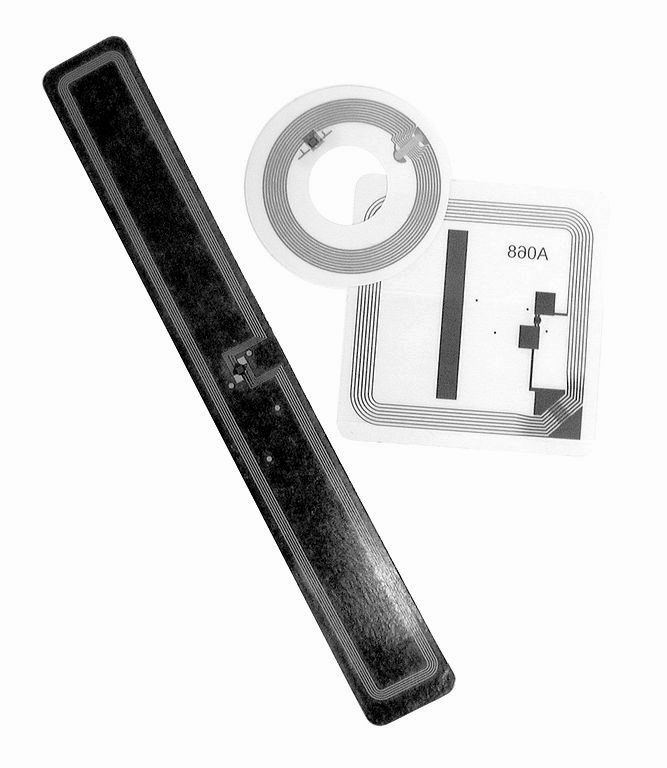
\includegraphics[width=\textwidth]{img/667px-RFID_Tags_gs.png}
                 \vspace{.1cm}
                 \caption{ RFID- Transponder}
                 \label{fig:TAGS}
         \end{subfigure}
%         
\qquad
%
         \begin{subfigure}[h]{0.4\textwidth}
                 \centering
                 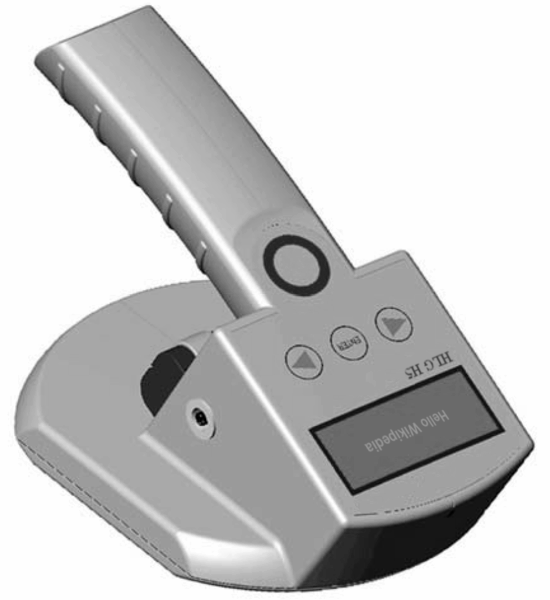
\includegraphics[width=\textwidth]{img/RFID-Reader_gs.png}
                 \vspace{.1cm}
                 \caption{RFID- Handlesegerät }
                 \label{fig:READER}
         \end{subfigure}
\end{figure}
%
\label{sec:Measurement1}
%
%

In der EU sind verschiedene RFID-Frequenzen zulässig, sie reichen von $865,0$ MHz bis $868,0$ MHz~\cite{etsi1}. Man kann damit die Wellenlänge mit: $ \lambda\simeq0,35 m $ angeben. Daraus folgt, dass alle 35 cm die gleiche Konfiguration der Phase vorliegt. Man spricht auch von \textit{Isophasen}. Daraus folgt, dass die gewonnene Information aus der Phase ist nicht eindeutig ist. Das bedeutet es lässt sich durch die Kenntnis der Phase nicht unmittelbar auf die korrekte Postion des Tags schließen. Man kann das Problem umgehen in dem man auf die errechnete Position ein ganzzahliges Vielfaches der Wellenlänge addiert, siehe Gleichung~\ref{eq:Phase_Wavenumber}. Die dort beschriebene Konstante $n$ wird Wellenzahl genannt.\\
%

Das System der \amedogmbh verwendet eine spezielle Antennenanordnung um die Position zu ermitteln. Dabei wird eine Antennenanzahl >4 eingesetzt. Für jede dieser Antennen muss eine eigene Wellenzahl bestimmt werden. Durch Auslöschung des Signals, Absorption etc. kann es dazu kommen, dass eine Antenne eine unbestimmte Zeit lang kein Signal vom Tag empfängt. Wenn die Antenne nach dieser Zeit erneut ein Signal empfängt ist die ihr zugehörige Wellenzahl unbekannt und muss neu bestimmt werden. \\
%

In realen Umgebungen treten zusätzlich noch Reflektionen auf, durch die ein sog. Multipath-Effekt entsteht. Dabei kann sein Signal den Reader auch über einen nicht direkten Weg erreichen und z.B. von Wänden oder Decken zurück auf die Antenne treffen. Das Signal wird nicht auf dem direkten Weg (Antenne->Tag->Antenne) empfangen sondern über einen unbekannten, längeren Weg. Darüber hinaus kann es in einer solchen Umgebung zu Auslöschungen und Verstärkungen kommen. Man stelle sich dazu ein Becken voller Wasser vor, genauer die Wellenausbreitung. Die Polarisation der Antennen begünstigt Auslöschung und Verstärkung zusätzlich. Es kommt es zu einem Fehler in der Phase und zu einer falschen Positionsberechnung. Die Fehlerbetrachtung ist nicht Gegenstand dieser Arbeit und wurde in anderen Arbeiten bereits behandelt z.B.~\cite{Borgwerth1}.
%

\subsection{PRPS-Messystem}
%
\begin{floatingfigure}[hr!]{7cm}
         \centering
         \caption[PRPS der \amedogmbh]{Abgebildet ist der Messaufbau aus vier Antennen. In dem Aufbau verbaut sind die wesentlichen elektronischen Komponenten wie Auswerte- und Steuereinheit. Nicht einzeln gezeigt.}
         \vspace{2mm}
         \label{fig:System}
         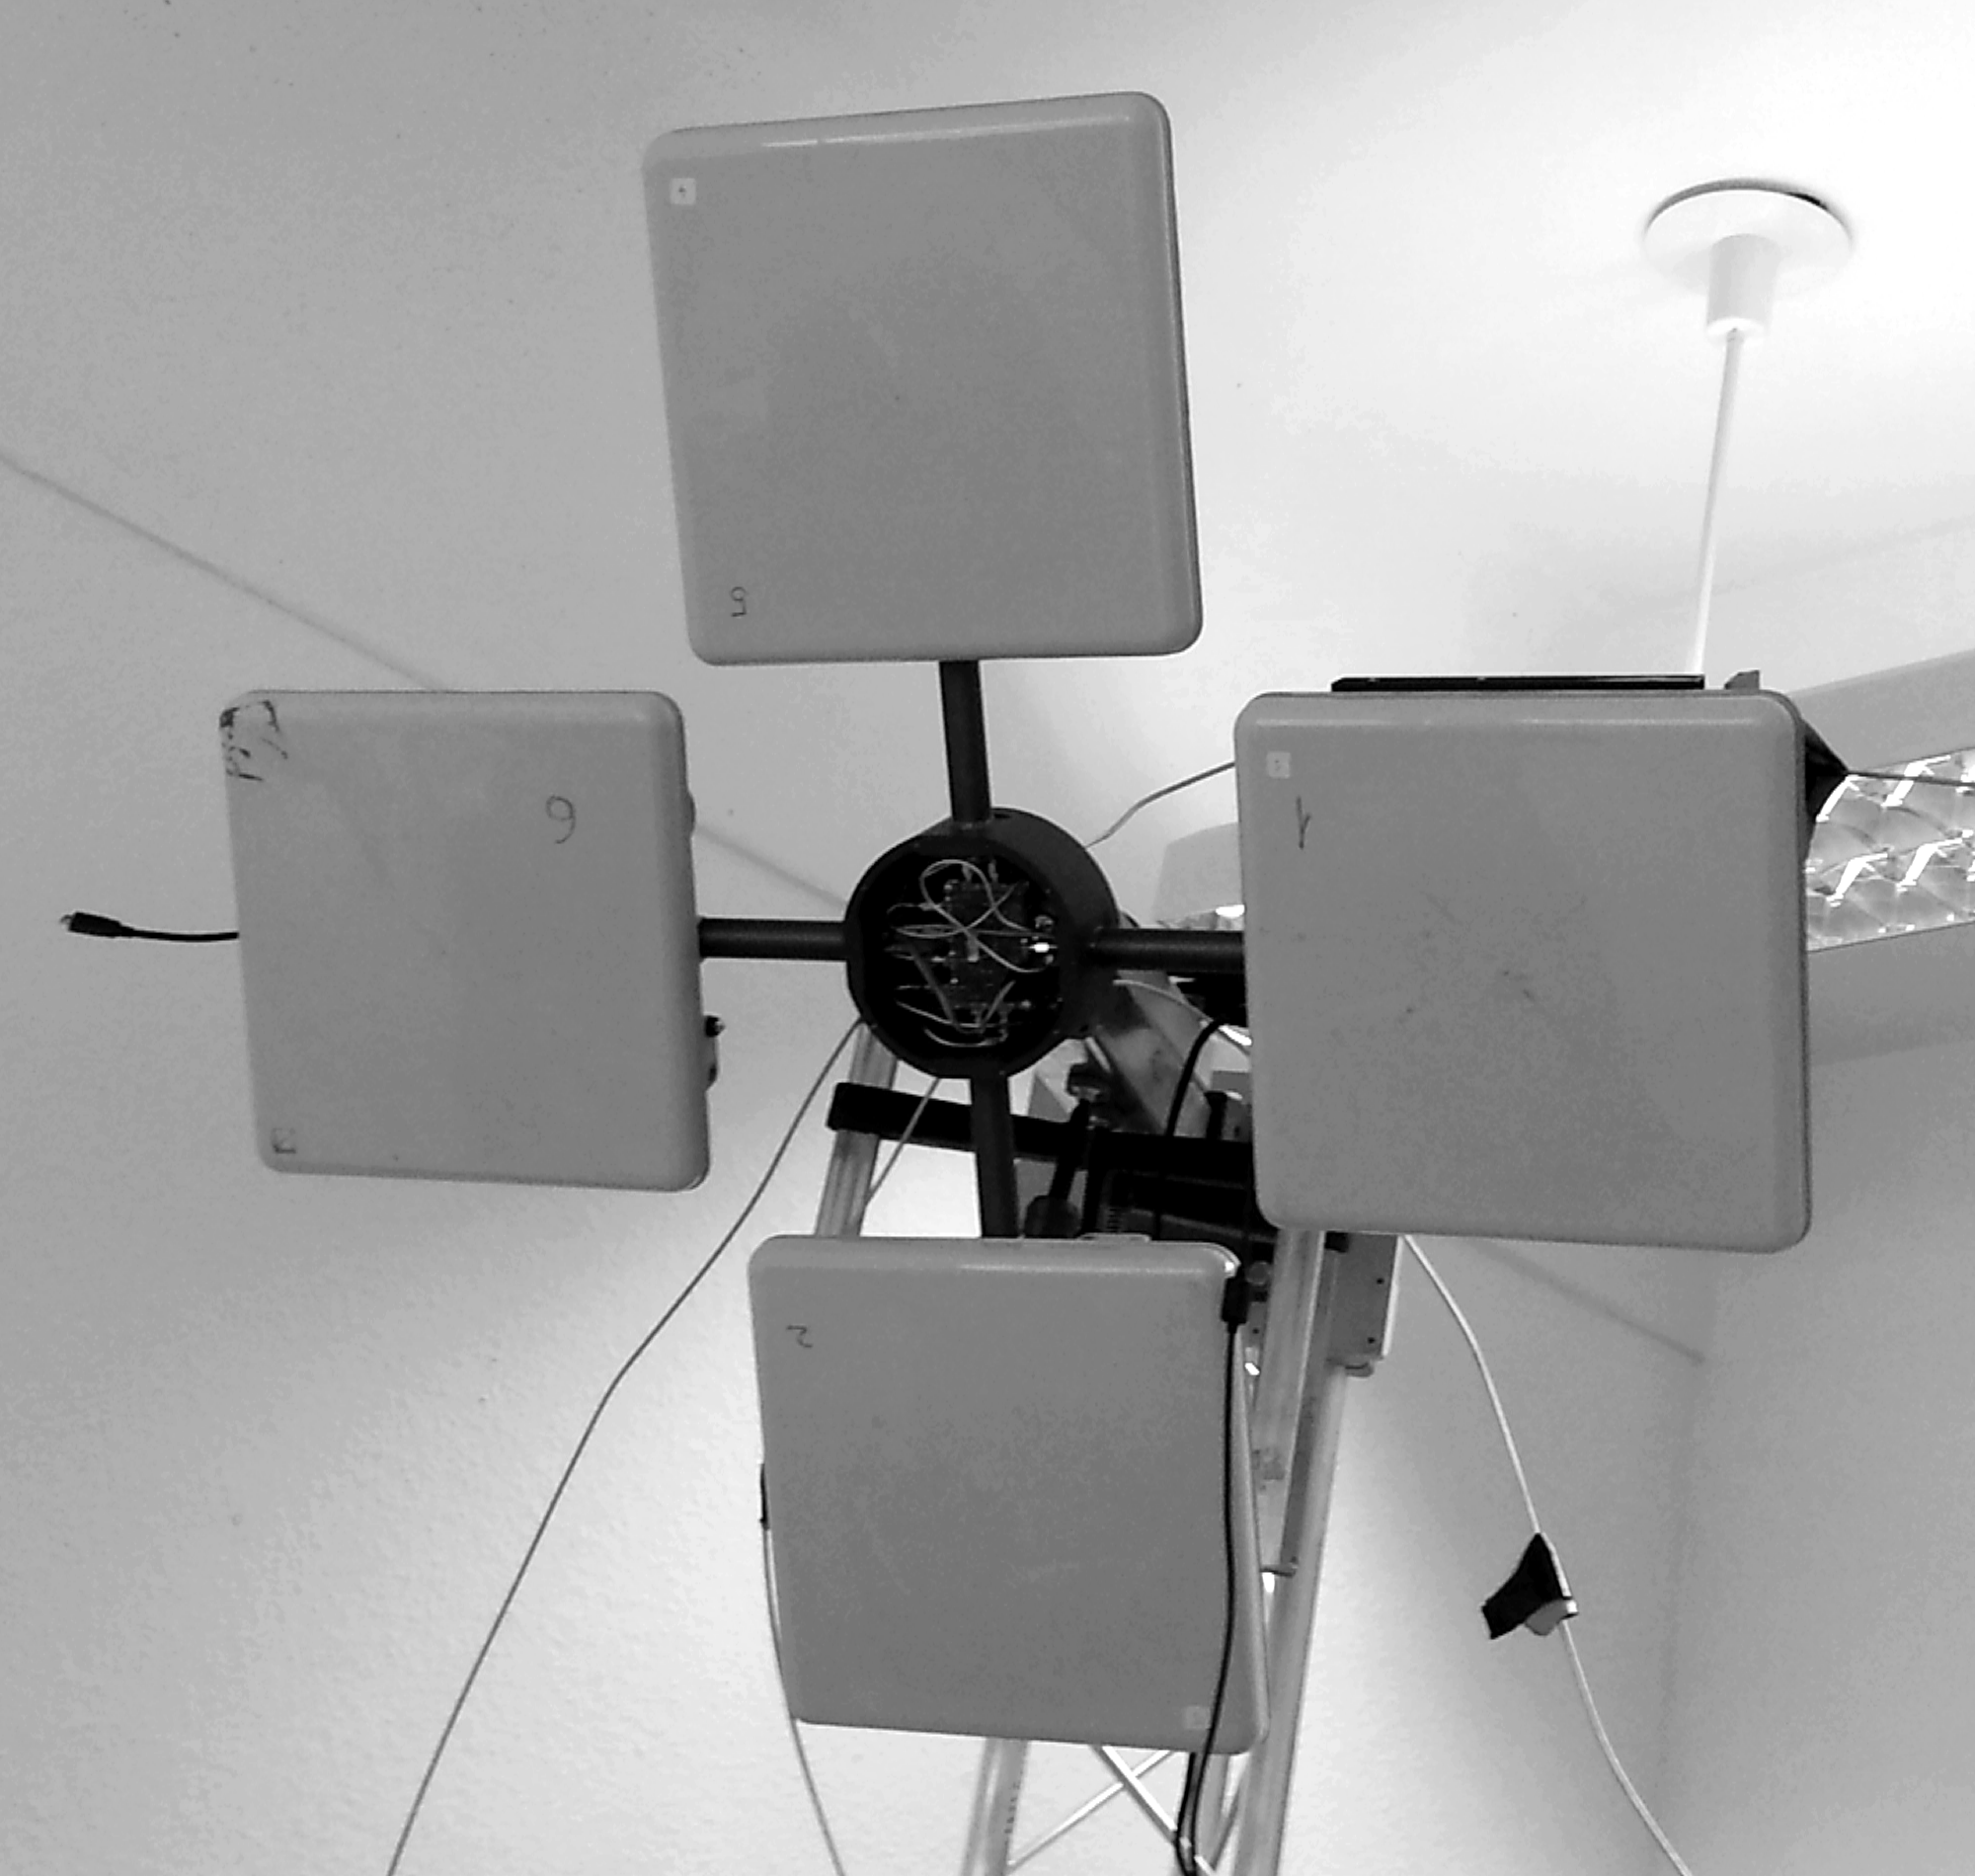
\includegraphics[width=0.4\textwidth]{img/4AntennaSetup_small.png}
         \vspace{2mm}
%         
\end{floatingfigure}
%
Das in dieser Arbeit Entwickelte Verfahren wird für das Messsystem der \amedogmbh entwickelt. Die Entwicklung wird Teil der Softwarekomponenten des Systems werden. Aktuelle befindet sich das gesamte System in der Revision, in diesem Abschnitt wird der Stand der Entwicklung dargestellt. Details über Hardware und Software werden im Rahmen der Arbeit nicht besprochen, sofern sie diese Arbeit nicht unmittelbar betreffen. \\
%

Das auf RFID basierende PRPS (Passiv RFID Positioning System) besteht aus mehreren frei positionierbaren Antennen, einer Mess- und Steuereinheit, sowie einem Rechner zur Kommunikation mit Endkundensoftware. Die Systemkomponenten für die Messwertaufnahme und Steuerung sind in einem Gehäuse untergebracht, dieses zeigt Abbildung~\ref{fig:System}. Eine typische Installation ist in Abbildung~\ref{fig:Setup} gezeigt. Dort wurde ein System mit insgesamt acht Antennen installiert. Vier Antennen sind frei aufgestellt, vier Weitere in einer festen Anordnung (\textit{Spinne}) installiert. Der Aufbau ist auf ein Messvolumina gerichtet.\\
%
\subsubsection{Leistungsmerkmale}
%
Das PRPS erlaubt eine Identifikation mehrerer Objekte oder genauer: RFID-Tags, die auf den Objekten angebracht sind. Wird ein einzelner Tag ausgewählt, kann seine Postion mit einer einer sehr hohen Frequenz ausgegeben werden. Die momentan Erreichbare Werte liegen bei $60$~Hz. Je nach Umgebung kann dieser Wert jedoch Variieren, siehe Kapitel~\ref{sec:Komplexity1}. Sollen mehrere Tags ausgegeben werden, verringert sich die Frequenz entsprechend. Bei der Verwendung von drei Tags ist eine Leserate von $20$~Hz pro Tag realistisch. Die Positionsgenauigkeit liegt aktuell bei $\approxeq 5$~mm. Die Antennen können frei Arrangiert werden. Das erlaubt eine Anpassung an nahezu jeden Raum und jeden Kundenbedarf. Als Tags kommen alle handelsüblichen RFID-Tags im verwendeten Frequenzband im Bereicht der ETSI-Frequenzen~\cite{etsi1} in Frage. Der Messbereich liegt bei mehreren Kubikmetern und einer erprobten maximalen Entfernung von $6-7$~Metern. Theoretisch ist das maximale Volumen noch größer. Die leistungstarke Messeinheit besteht aus einer sehr flexiblen Messelektronik. Diese ist in der Lage eine sehr hohe Güte und Frequenz der Messwerte zu realisieren.\\

%
\begin{figure}[h]
         \centering
         \caption[PRPS der amedo GmbH]{Abgebildet ist der Messaufbau mit unterschiedlichen Antennen. Der Aufbau ist auf ein Messvolumina von mehreren Kubikmetern ausgerichtet}
		\label{fig:Setup}
		\vspace{2mm}
         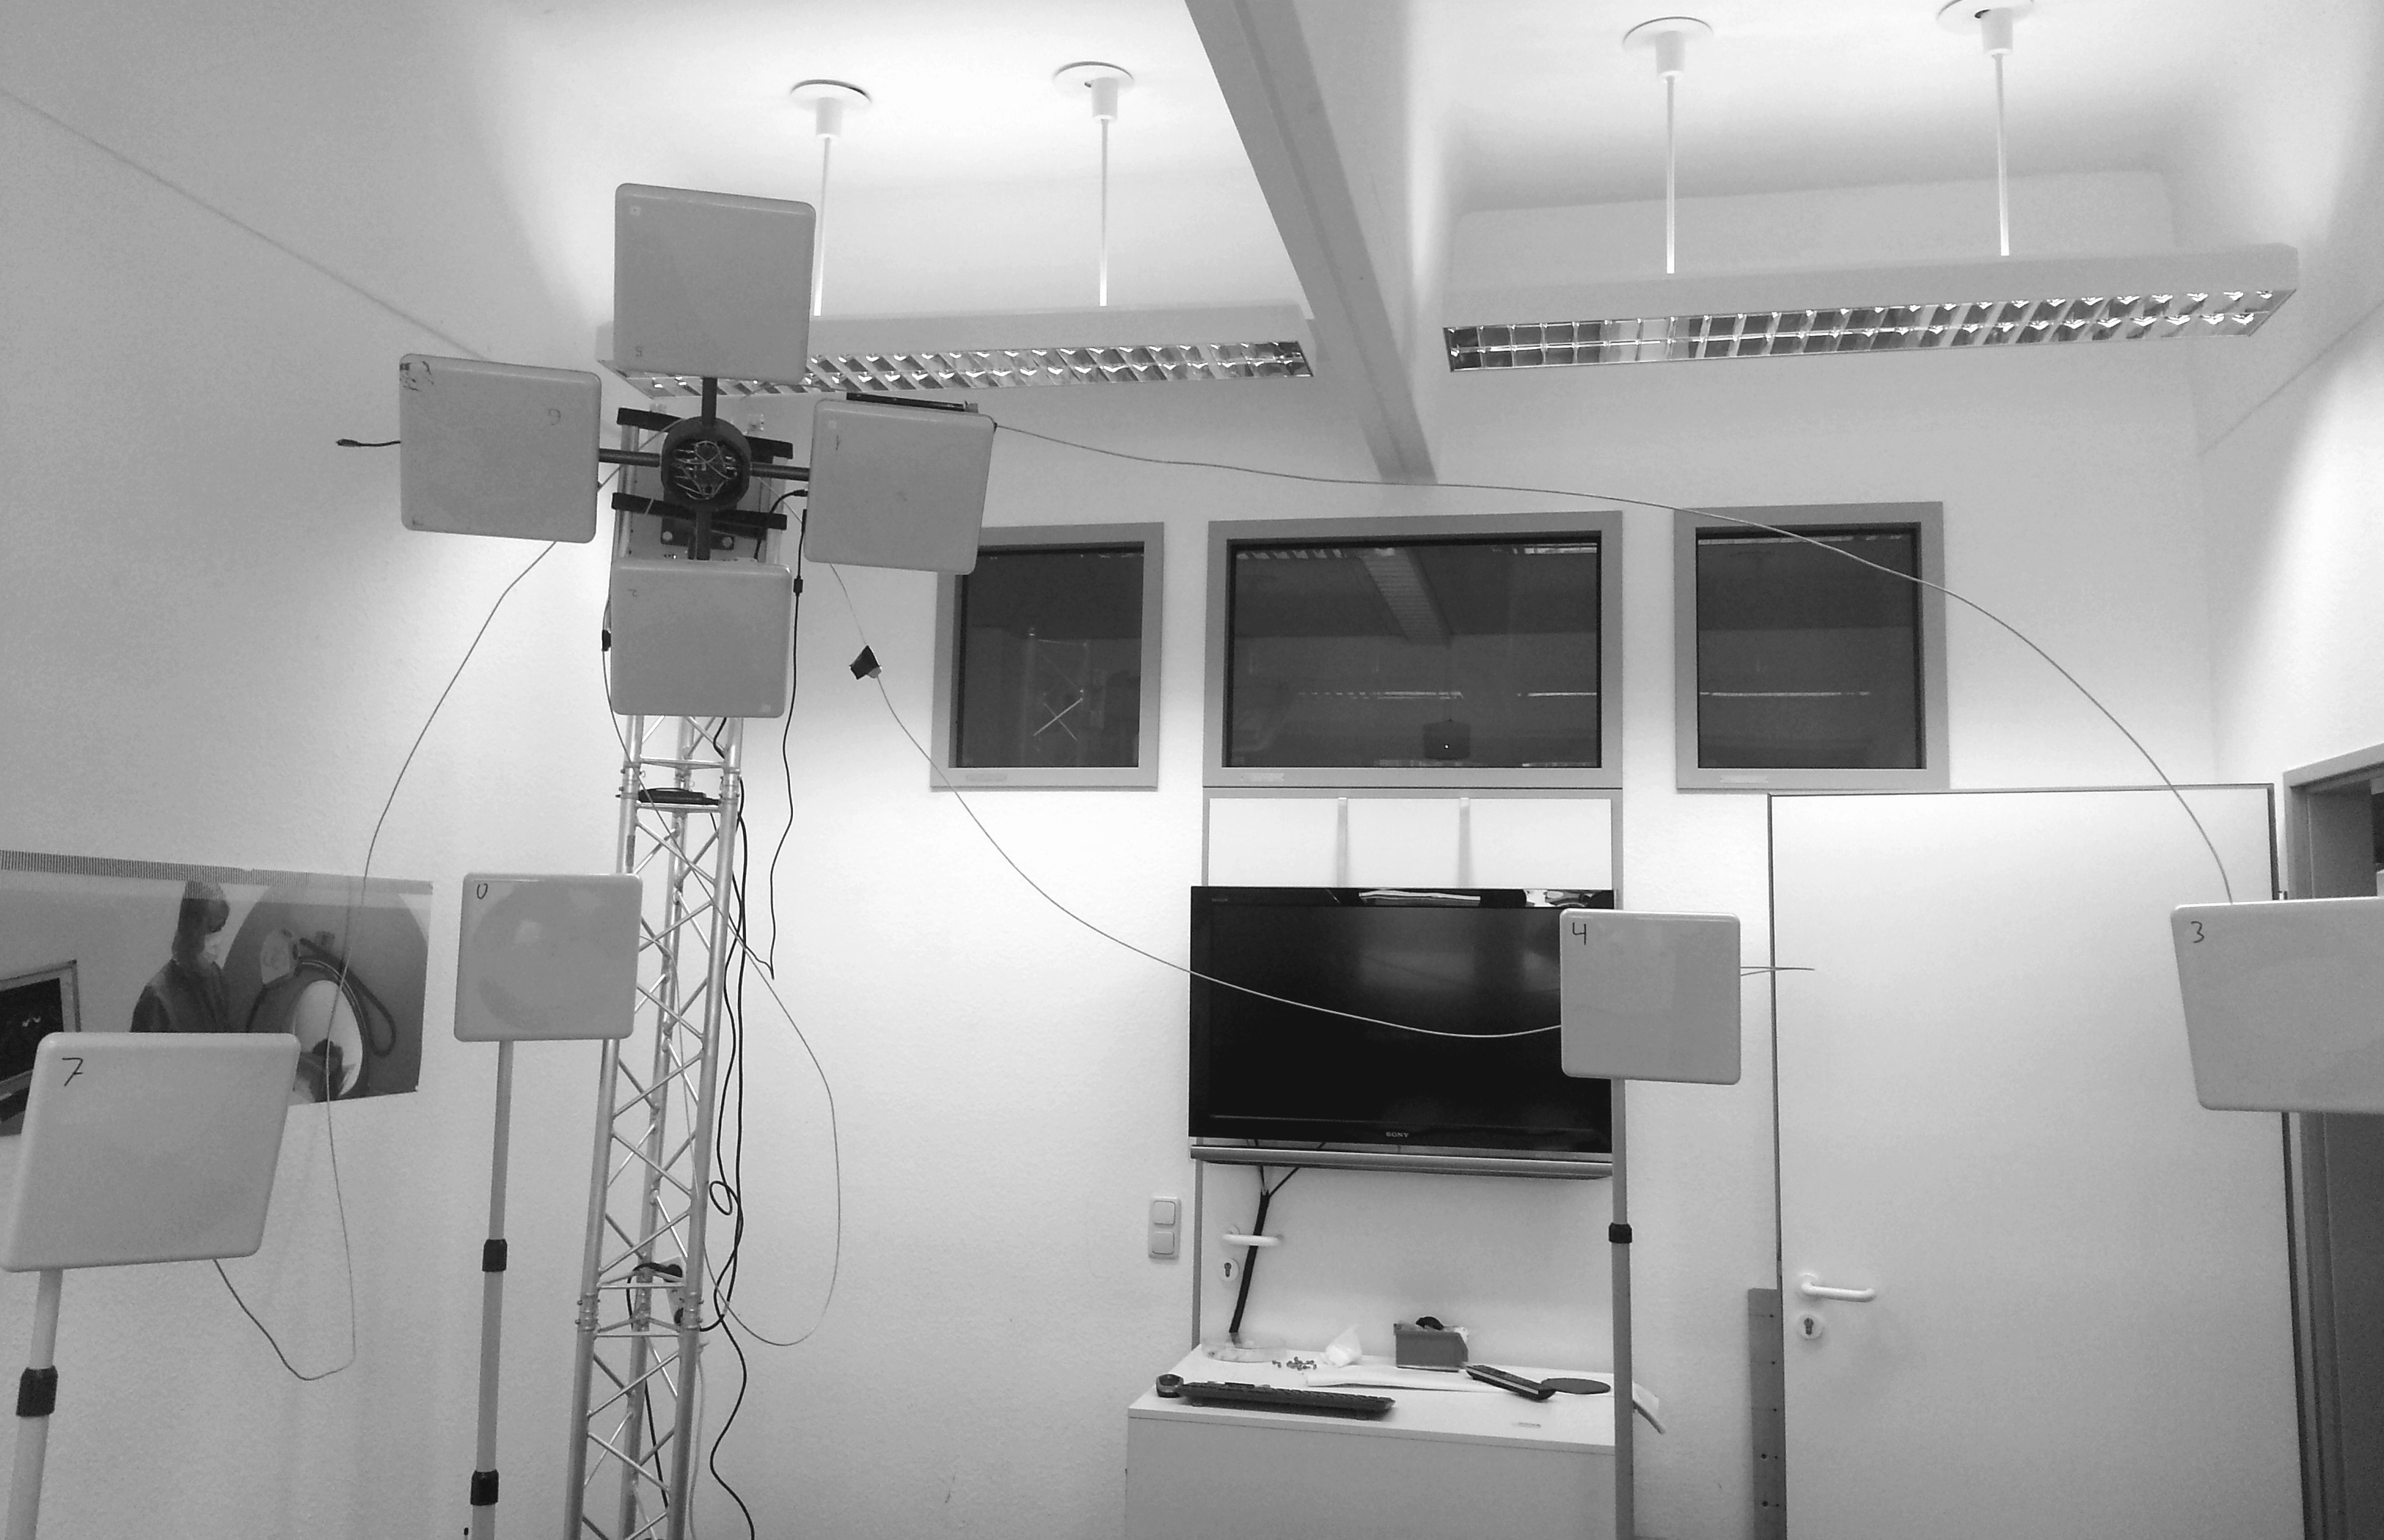
\includegraphics[width=\textwidth]{img/RFID-Okto.png}
         
\end{figure}
%

\subsection{Phase und Wellenzahl}
\label{sec:wavenumber}
\begin{figure} [h]
\centering
         \caption[Zusammenhang Wellenlänge - Wellenzahl]{Dargestellt ist der Zusammenhang zwischen der Wellenlänge $\lambda$ und der Wellenzahl $n$. Da die Phase alle $2\pi$ den gleichen Wert annimmt, wird mit dem Faktor $n$ ein vielfaches der Wellenlänge aufaddiert. Dadurch erhält man die Entfernung zu dem Tag.}
         \label{fig:wavenumber_wavelength}
         \vspace{0.5cm}
         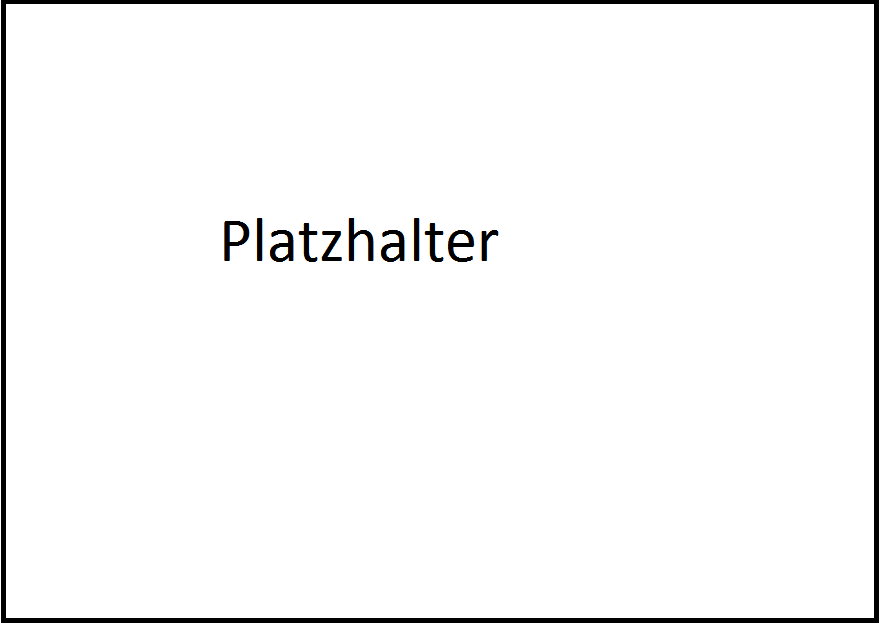
\includegraphics[width=\textwidth]{img/00_placeholder.png}
%      
\end{figure}

Aus der Abbildung~\ref{fig:wavenumber_wavelength} lässt sich folgender Zusammenhang ableiten.
%
\begin{equation}
\label{eq:Phase_Wavenumber}
	d(\Theta, n)=\lambda(\Theta+n)
\end{equation}

\lipsum[1]
%